\documentclass[12pt]{article}
\usepackage[margin=5cm]{geometry} 
\usepackage{amsmath,amsthm,amssymb,amsfonts, fancyhdr, color, comment, graphicx, environ}
\usepackage{xcolor}
\usepackage{mdframed}
\usepackage[shortlabels]{enumitem}
\usepackage{indentfirst}
\usepackage{hyperref}
\usepackage{tensor}

\usepackage{logicproof}

\usepackage{graphicx}
\graphicspath{ {./images/} }

\hypersetup{
    colorlinks=true,
    linkcolor=blue,
    filecolor=magenta,      
    urlcolor=blue,
}
\usepackage{tikz-cd}
\tikzset{ampersand replacement = \&}
\pagestyle{fancy}

\usepackage{tikz}
\newcommand*\circled[1]{\tikz[baseline=(char.base)]{\node[shape=circle,draw,inner sep=1pt] (char) {#1};}}
            
    

\newenvironment{problem}[2][Problem]
    { \begin{mdframed}[backgroundcolor=gray!20] \textbf{#1 #2} \\}
    {  \end{mdframed}}

\newenvironment{solution}
    {{\textbf{Solution}}}

\def\boxit#1#2{%
    \smash{\color{red}\fboxrule=1pt\relax\fboxsep=2pt\relax%
    \llap{\rlap{\fbox{\phantom{\rule{#1}{#2}}}}~}}\ignorespaces
}

\newcommand\LL[1]{\multicolumn{1}{|c}{#1}}
\newcommand\RR[1]{\multicolumn{1}{c|}{#1}}
\newcommand\LR[1]{\multicolumn{1}{|c|}{#1}}
% \cline{2-7}


%%%%%%%%%%%%%%%%%%%%%%%%%%%%%%%%%%%%%%%%%%%%%%%
\usepackage{tikzpagenodes}
\usetikzlibrary{calc}

\makeatletter
\tikzset{%
  remember picture with id/.style={%
    remember picture,
    overlay,
    save picture id=#1,
  },
  save picture id/.code={%
    \edef\pgf@temp{#1}%
    \immediate\write\pgfutil@auxout{%
      \noexpand\savepointas{\pgf@temp}{\pgfpictureid}}%
  },
  if picture id/.code args={#1#2#3}{%
    \@ifundefined{save@pt@#1}{%
      \pgfkeysalso{#3}%
    }{
      \pgfkeysalso{#2}%
    }
  }
}

\def\savepointas#1#2{%
  \expandafter\gdef\csname save@pt@#1\endcsname{#2}%
}

\def\tmk@labeldef#1,#2\@nil{%
  \def\tmk@label{#1}%
  \def\tmk@def{#2}%
}

\tikzdeclarecoordinatesystem{pic}{%
  \pgfutil@in@,{#1}%
  \ifpgfutil@in@%
    \tmk@labeldef#1\@nil
  \else
    \tmk@labeldef#1,(0pt,0pt)\@nil
  \fi
  \@ifundefined{save@pt@\tmk@label}{%
    \tikz@scan@one@point\pgfutil@firstofone\tmk@def
  }{%
  \pgfsys@getposition{\csname save@pt@\tmk@label\endcsname}\save@orig@pic%
  \pgfsys@getposition{\pgfpictureid}\save@this@pic%
  \pgf@process{\pgfpointorigin\save@this@pic}%
  \pgf@xa=\pgf@x
  \pgf@ya=\pgf@y
  \pgf@process{\pgfpointorigin\save@orig@pic}%
  \advance\pgf@x by -\pgf@xa
  \advance\pgf@y by -\pgf@ya
  }%
}
\newcommand\tikzmark[2][]{%
\tikz[remember picture with \usepackage{logicproof}
id=#2] #1;}
\makeatother

\newcommand\BoxedText[3][]{%
\begin{tikzpicture}[remember picture,overlay]
\draw[#1] 
  let \p1=(pic cs:#2), \p2=(pic cs:#3) in
  ([yshift=-0.8ex]\p1) --
  ([yshift=2ex]\p1) -- 
  ([xshift=3pt,yshift=2ex]\p1-|current page text area.east) -- 
  ([xshift=3pt,yshift=2ex]\p2-|current page text area.east) --
  ([yshift=2ex]\p2) --
  ([yshift=-0.8ex]\p2) --
  ([xshift=-3pt,yshift=-0.8ex]\p2-|current page text area.west) --
  ([xshift=-3pt,yshift=-0.8ex]\p1-|current page text area.west) --
  cycle
;
\end{tikzpicture}%
}

\newcommand{\gradientbox}[2]{%
    \BoxedText[draw=orange!70!black,right color=orange!10,left color=orange!50]     {start#1}{end#1}
    \tikzmark{start#1}#2
    \tikzmark{end#1}
}

\newcommand{\shadedbox}[2]{%
    \BoxedText[draw=cyan!70!black,fill=cyan!30,ultra thick]{start#1}{end#1}
    \tikzmark{start#1}#2
    \tikzmark{end#1}
}

\newcommand{\outlinebox}[2]{%
    \BoxedText{start#1}{end#1}
    \tikzmark{start#1}#2
    \tikzmark{end#1}
}

\newcommand{\sentence}[4]{$^{\circled{#2}}${\BoxedText[draw=#3!70!black,fill=#3!15,thick]{start#1}{end#1}
    \tikzmark{start#1}#4
    \tikzmark{end#1}}}

\usetikzlibrary{arrows}
\usetikzlibrary{shapes}
\newcommand{\indicator}[1]{%
  \tikz[baseline=(char.base)]\node[anchor=south west, draw,rectangle, rounded corners, inner sep=2pt, minimum size=6mm,
    text height=2mm](char){\textbf{#1}} ;}






\newcommand{\ptext}[1]{\parbox{.9\textwidth}{#1}}

\newcommand{\wff}
{Well Formed Formula }

\def\checkmark{\tikz\fill[scale=0.4](0,.35) -- (.25,0) -- (1,.7) -- (.25,.15) -- cycle;} 

%%%%%%%%%%%%%%%%%%%%%%%%%%%%%%%%%%%%%%%%%%%%%
\lhead{PHIL131.01 \\ Assignment-7}
\rhead{Atahan \\ Haznedar} 
\chead{\textbf{2021107075}}
%%%%%%%%%%%%%%%%%%%%%%%%%%%%%%%%%%%%%%%%%%%%%


\begin{document}
    \section*{Chapter 5}
    \paragraph{I}
    Some of the following arguments can be formalized as immediate inferences involving a pair of categorical statements or as categorical syllogisms; others cannot. Formalize those which can and test the resulting forms for validity with Venn diagrams
    

    \begin{problem}{1}
        No one has conquered the world. Therefore, it is not true that someone has conquered the world.
    \end{problem}
    
    \begin{solution}
        P: 'People' & C: 'things that have conquered the world'
        
        \begin{tabular}{l l l}
             & No P are C. \\
             $\therefore$ & $\sim$(Some P are C.) \\
        \end{tabular}
        
        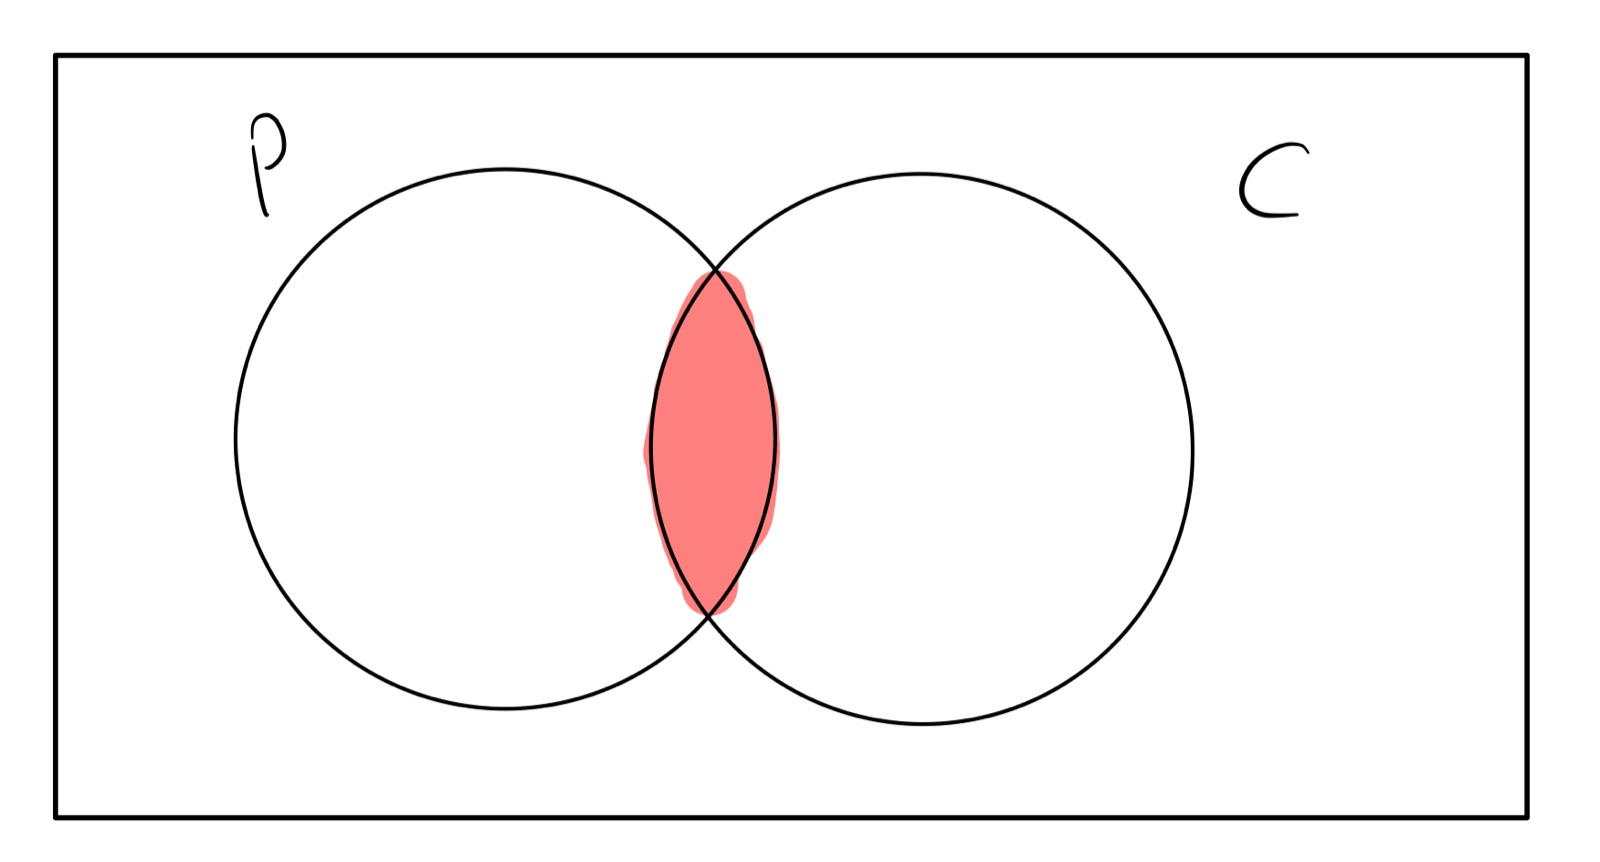
\includegraphics[width=8cm,height=4cm]{Q1}
    
        So it is Valid.
    \end{solution}
  
\clearpage

    \begin{problem}{2}
        No one has conquered the world. Therefore, not everyone has conquered the world.
    \end{problem}

    \begin{solution}
        P: 'People' & C: 'things that have conquered the world'
        
        \begin{tabular}{l l l}
             & No P are C. \\
             $\therefore$ & $\sim$(All P are C.) \\
        \end{tabular}
          
        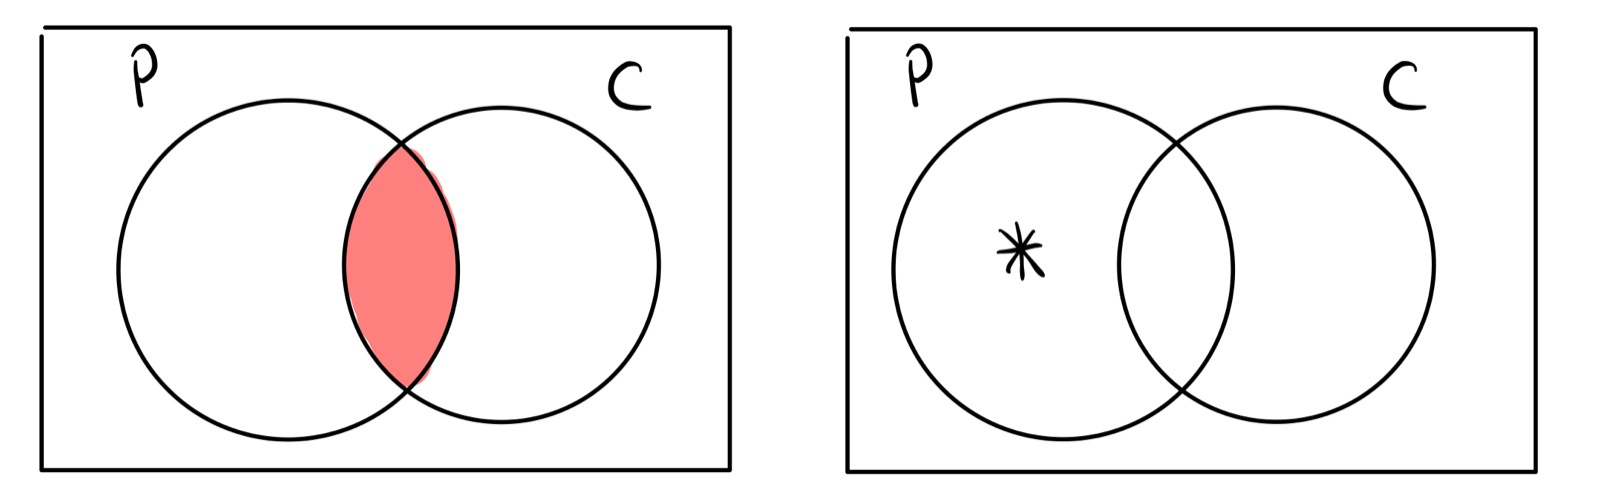
\includegraphics[width=12cm,height=4cm]{Q2}
        
        It is invalid.
    \end{solution}



    \begin{problem}{6}
        All square numbers are nonprime. So all prime numbers are nonsquare.
    \end{problem}
    
    \begin{solution}
        S: 'Square Numbers' & P: 'Prime Numbers'
        
        \begin{tabular}{l l l}
             & All S are non-P. \\
             $\therefore$ & All P are non-S. \\
        \end{tabular}
        
        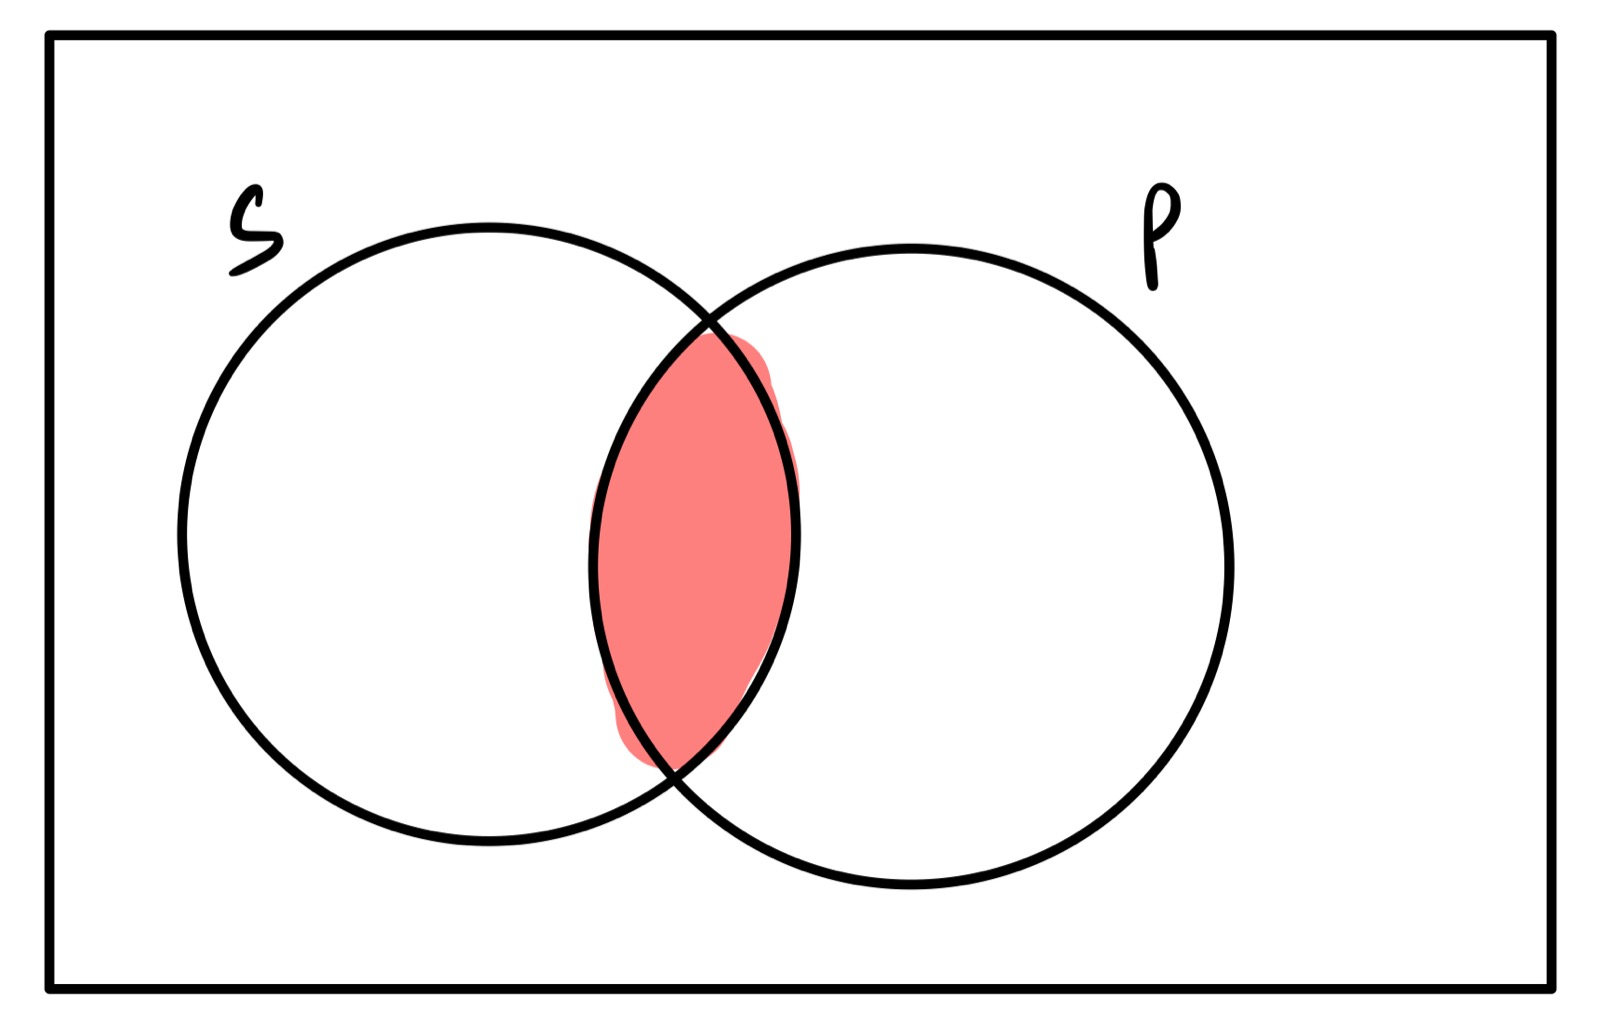
\includegraphics[width=8cm,height=4cm]{Q6}
         
        Hence it is Valid
        
        
    \end{solution}    
    
    
    
    
    \begin{problem}{9}
        No arms control agreement will be reached now. So no arms control agreement will be reached at any other time.
    \end{problem}
    
    
    \begin{solution}
        R: 'Thing that will be reached now' & A: 'Armscontrol agreement'
        
        \begin{tabular}{l l l}
             & No A are R. \\
             $\therefore$ & No A are non-R. \\
        \end{tabular}
        
        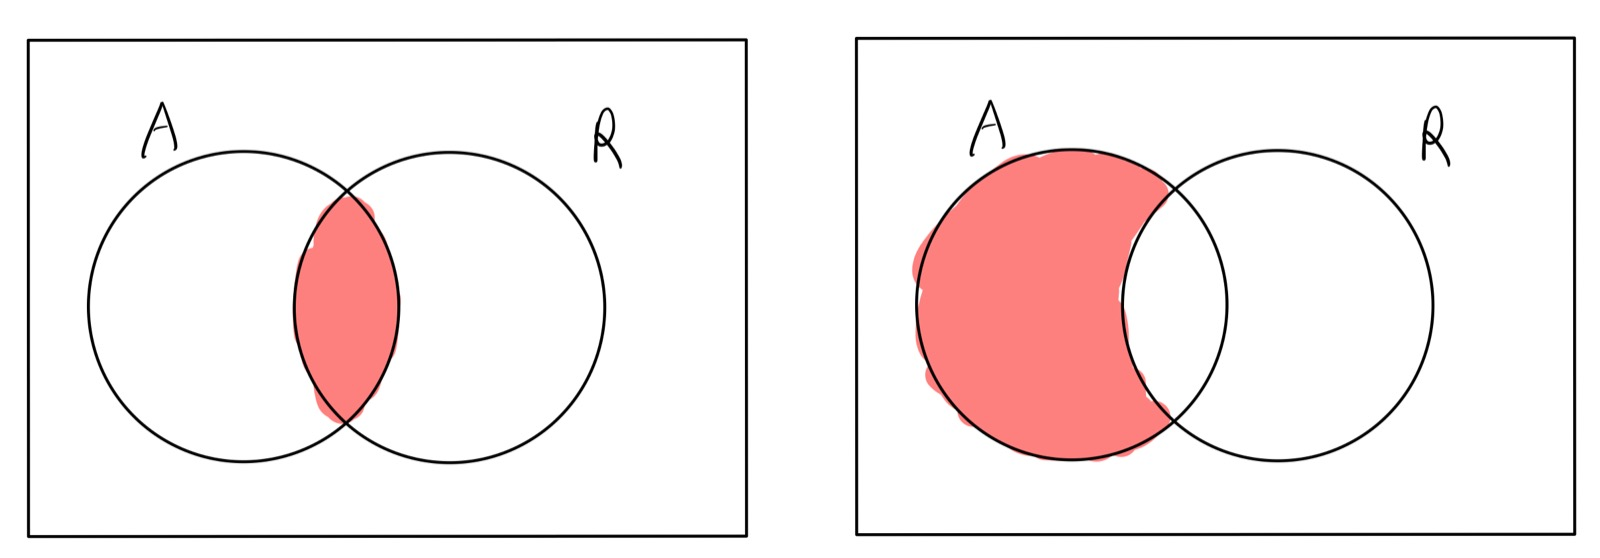
\includegraphics[width=12cm,height=4cm]{Q9}
         
        Hence it is invalid.
        
        
    \end{solution}

    \begin{problem}{13}
        If Jean is sick, she won’t come to work. If she doesn’t come to work, none of us will have anything to do. So if Jean is sick, none of us will have anything to do.
    \end{problem}
  
  
    \begin{solution}
        It is not a categorical argument. However it is valid because of the transivity of a conditional.     
    \end{solution}  
  
\clearpage  
  
    
    \begin{problem}{14}
        Some people are nonsmokers. Some are nondrinkers. Therefore, some nonsmokers are non-drinkers.
    \end{problem}
    
    
    \begin{solution}
        P: 'People' & S: 'nonsmokers' & D: 'nondrinkers'
        
        \begin{tabular}{l l l}
             & Some P are S\\
             & Some P are D \\
             $\therefore$ & Some S are D \\
        \end{tabular}
        
        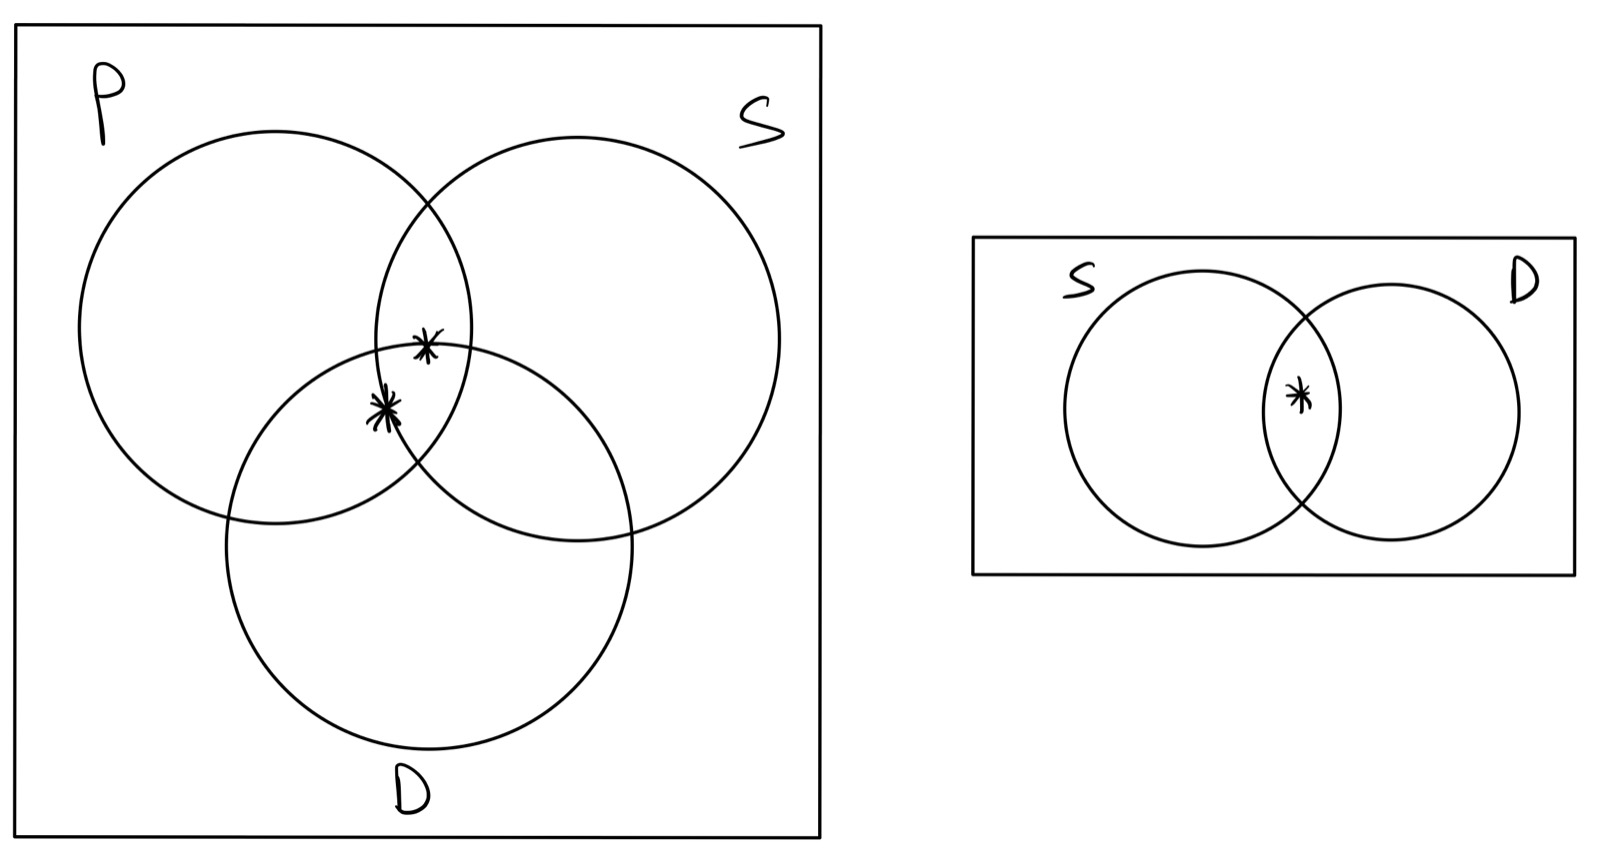
\includegraphics[width=10cm,height=6cm]{Q14}
         
        Hence it is invalid.        
    \end{solution}

\clearpage    
    
    \begin{problem}{17}
        All good things must pass. No dictatorship is a good thing. Consequently, some dictatorships do not pass.
    \end{problem}

    \begin{solution}
        P: 'things that must pass' & D: 'Dictatorship' & G: 'things that are good'
        
        \begin{tabular}{l l l}
             & All G are P\\
             & No D are G \\
             $\therefore$ & Some D are not P \\
        \end{tabular}
        
        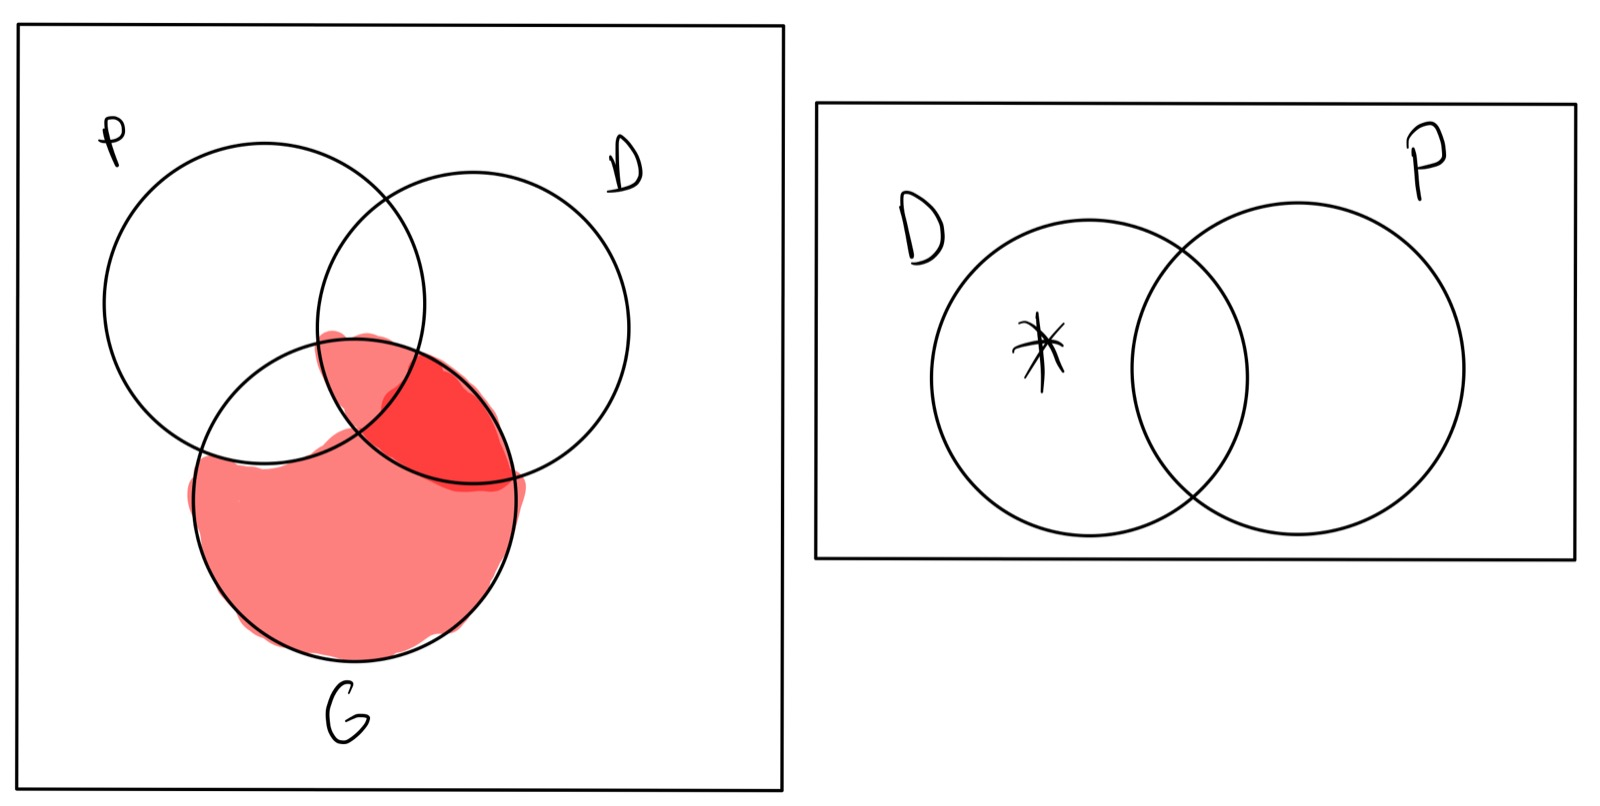
\includegraphics[width=12cm,height=4cm]{Q17}
         
        Hence it is invalid.        
    \end{solution}

\clearpage    
    
    \begin{problem}{19}
        Every electron has a negative charge. No positron has a negative charge. Therefore some positrons are not electrons.
    \end{problem}

    \begin{solution}
        E: 'Electron' & N: 'things that have negative charge' & P: 'Positron'
        
        \begin{tabular}{l l l}
             & Every E are N \\
             & No P are N \\
             $\therefore$ & Some P are not E \\
        \end{tabular}
         
        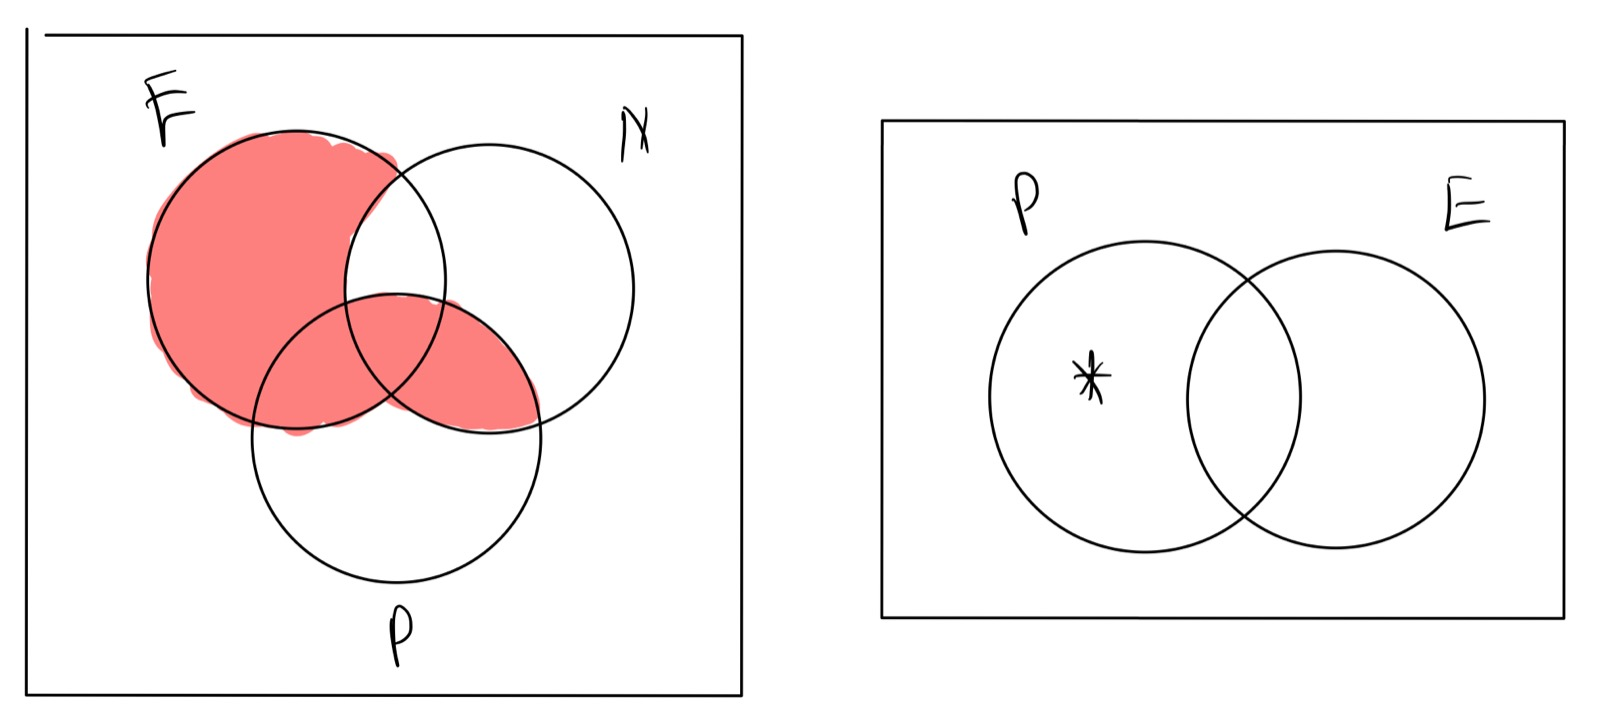
\includegraphics[width=12cm,height=4cm]{Q19}
        
        Hence it is invalid.        
    \end{solution}    
    
    
    
    
    
    
\end{document}